\subsubsection{Jet Identification}

Jets are reconstructed by using the anti-$k_T$ clustering algorithm out of particle flow candidates, with a distance parameter $R = 0.4$, 
after rejecting the charged hadrons that are associated to a pileup primary vertex.

To reduce instrumental background, the tight working point jet ID suggested by the JetMET Physics Object Group is applied.%~\cite{JetID2018}. 
In addition, jets from Pile-Up are rejected using the PileUp jet ID criteria suggested by the JetMET POG.%~\cite{JetPUID2017}.
It is to be noted that the PU JetID was only derived for 2016 conditions but is also applied to 2017 and 2018 samples. 

In this analysis, the jets are required to be within $|\eta| < 4.7$ area and have a transverse momentum above 30 GeV. 
In addition, the jets are cleaned from any of the tight leptons (passing the SIP and isolation cut computed after FSR correction) 
and FSR photons by a separation criterion: $\Delta R(\text{jet,lepton/photon}) > 0.4$.
\\
In addition this analysis considers also a collection of large radius jets clustered using the same anti-$k_T$ algorithm with a distance parameter $R = 0.8$.
These jets are cleaned using the Pileup Per Particle Identification (PUPPI) \cite{Bertolini_2014}, which is a method for pileup mitigation.

\subsubsection{Jet Energy Corrections}

The calorimeter response to particles is not linear
and it is not straightforward to translate the measured jet energy
to the true particle or parton energy, therefore Jet Energy Corrections must be applied.
In this analysis, standard jet energy corrections are applied to the reconstructed jets,
which consist of L1 Pileup, L2 Relative Jet Correction,
L3 Absolute Jet Correction for both Monte Carlo samples and data,
and also residual calibration for data%.~\cite{JECMC2018}. 

Jet corrections are applied following JetMET Physics Object Group recommendations. The corrections used are as follows:
\begin{itemize}
\item Jet energy scale corrections for data
\begin{itemize}
\item 2016: Summer19UL16\_RunBCDEFGH\_Combined\_V7\_DATA\_AK4PFchs
\item 2017: Summer19UL17\_RunBCDEF\_V5\_DATA\_AK4PFchs
\item 2018: Summer19UL18\_V5\_DATA\_AK4PFchs
\end{itemize}
\item Jet energy scale corrections for MC
\begin{itemize}
\item 2016preVFP: Summer19UL16APV\_V7\_MC\_AK4PFchs
\item 2016postVFP: Summer19UL16\_V7\_MC\_AK4PFchs
\item 2017: Summer19UL17\_V5\_MC\_AK4PFchs
\item 2018: Summer19UL18\_V5\_MC\_AK4PFchs
\end{itemize}
\item Jet energy resolution corrections
\begin{itemize}
\item 2016preVFP: Summer20UL16APV\_JRV3\_MC\_[Pt/Phi]Resolution\_AK4PFchs
\item 2016postVFP: Summer20UL16\_JRV3\_MC\_[Pt/Phi]Resolution\_AK4PFchs
\item 2017: Summer19UL17\_JRV3\_MC\_[Pt/Phi]Resolution\_AK4PFchs
\item 2018: Summer19UL18\_JRV2\_MC\_[Pt/Phi]Resolution\_AK4PFchs
\end{itemize}
\end{itemize}

% \textbf{At the moment only preliminary version of JEC for MC is available. As recommended no JEC is applied to data.}
%Jet Energy Resolutions corrections are, however, NOT applied to 2018 samples (see discussion below).

\paragraph{L1 pre-firing}

In 2016 and 2017, the gradual timing shift of ECAL was not properly propagated to L1 trigger primitives (TP) resulting in a significant fraction of high eta TP being mistakenly associated to the previous bunch crossing.
Since Level 1 rules forbid two consecutive bunch crossings to fire, an unpleasant consequence of this (in addition to not finding the TP in the bx 0) is that events can self veto if a significant amount of ECAL energy is found in the region of $2.<|\eta|<3$.
This effect is not described by the simulations.%~\cite{L1PrefiringTwiki}.
The probability not to prefire is calculated for each event and applied as a weight to simulation for 2016 and 2017 samples.
The official tool is used for this purpose.%~\cite{L1PrefiringTwiki}.

\begin{figure}
\subfigure [L1 pre-firing weights]       {\resizebox{.5\textwidth}{!}{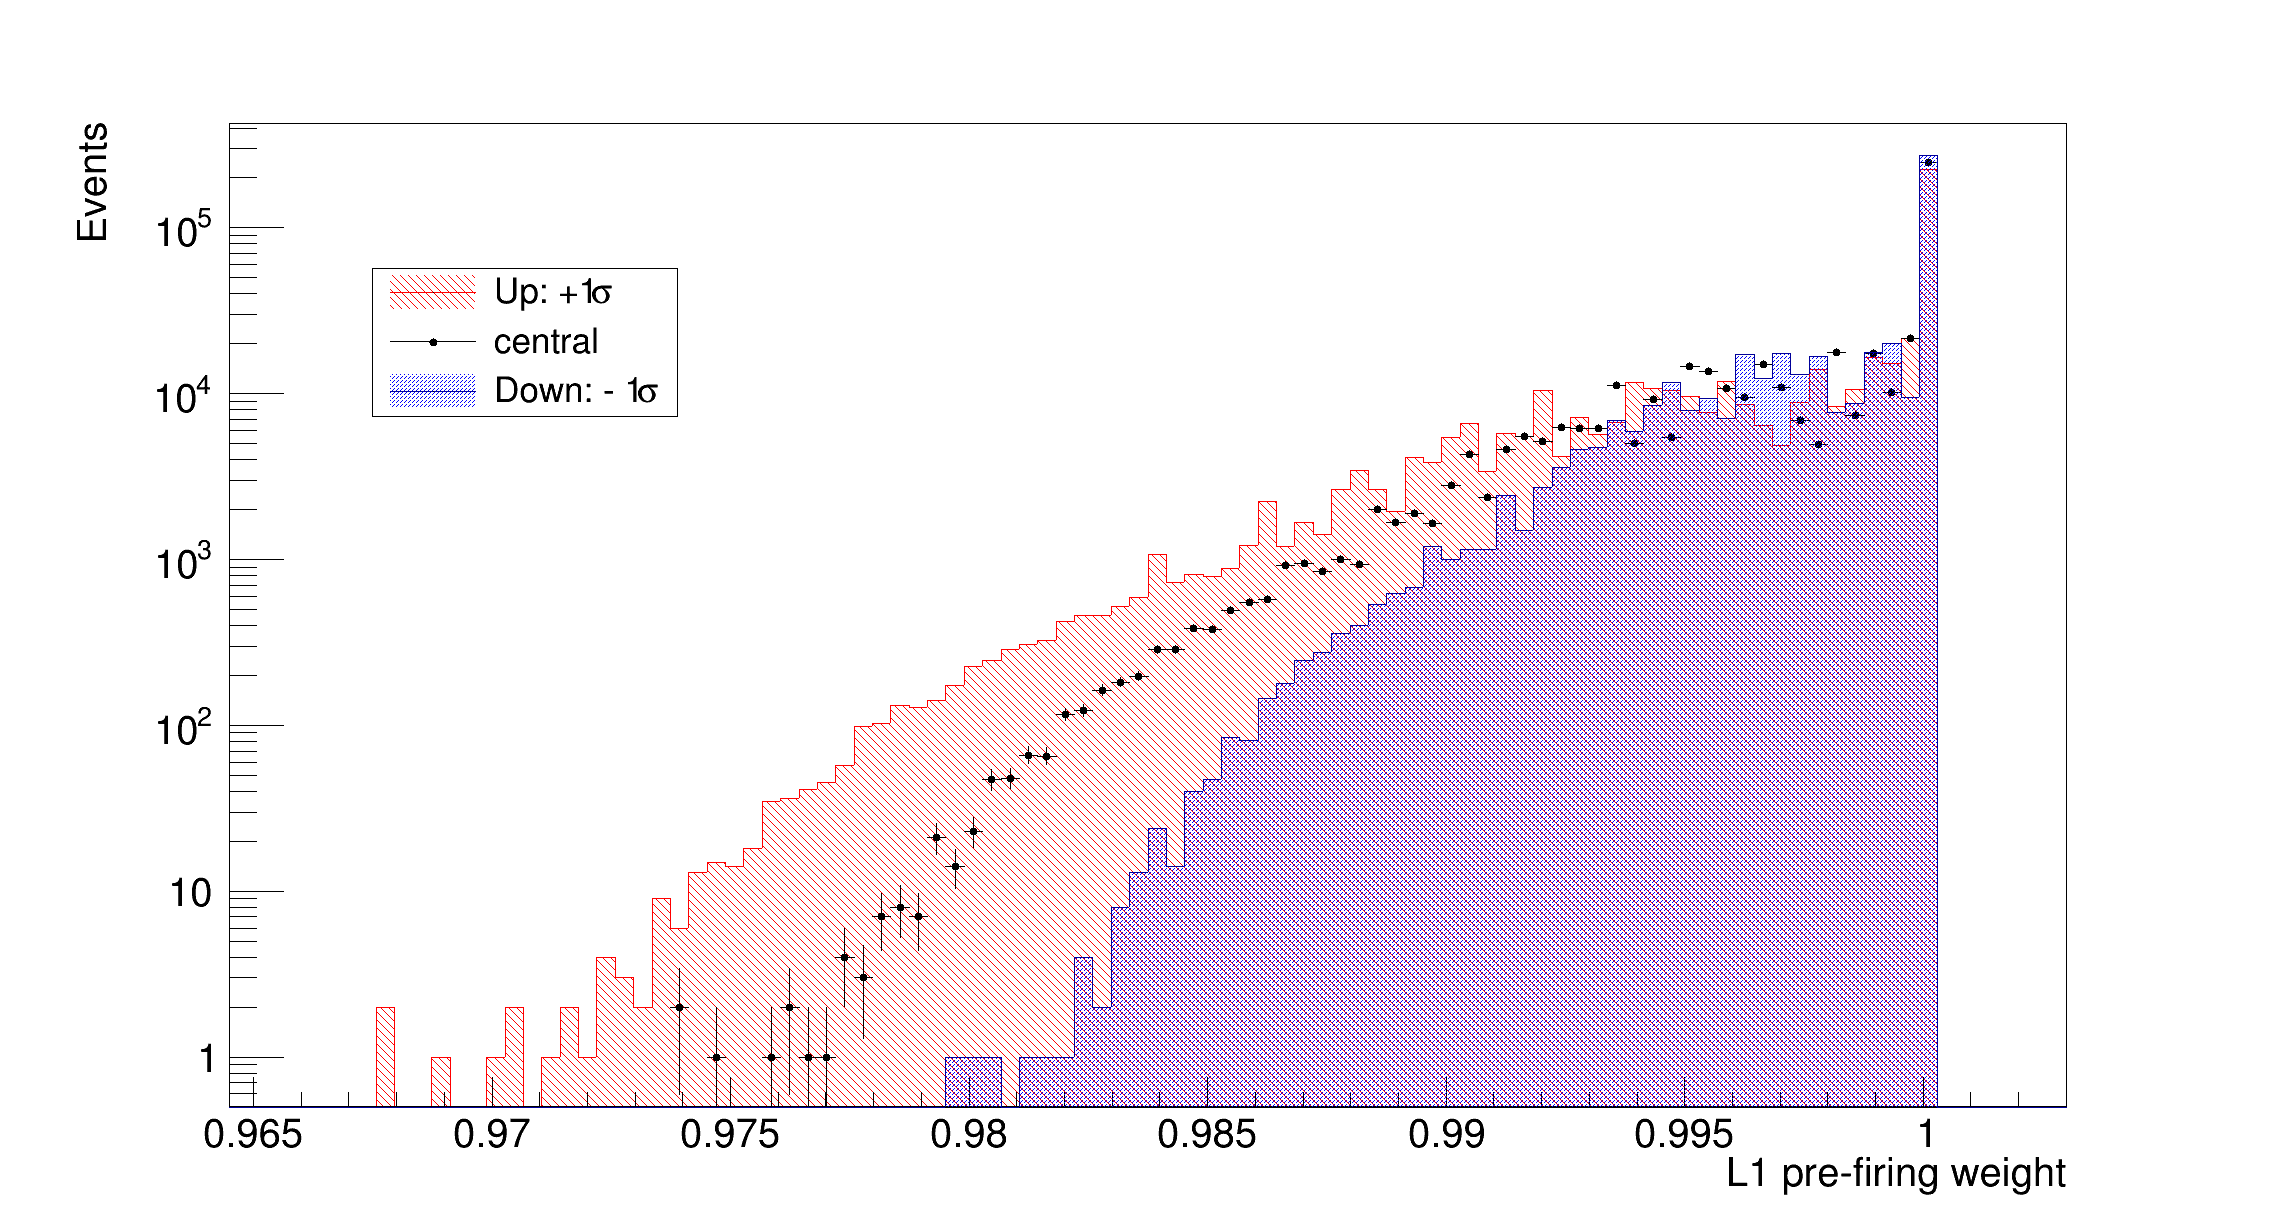
\includegraphics[width=.5\textwidth]{Figures/L1Prefiring_ZZGTo4LG.png}}}
\subfigure [Effect on $m_{4\ell\gamma}$] {\resizebox{.5\textwidth}{!}{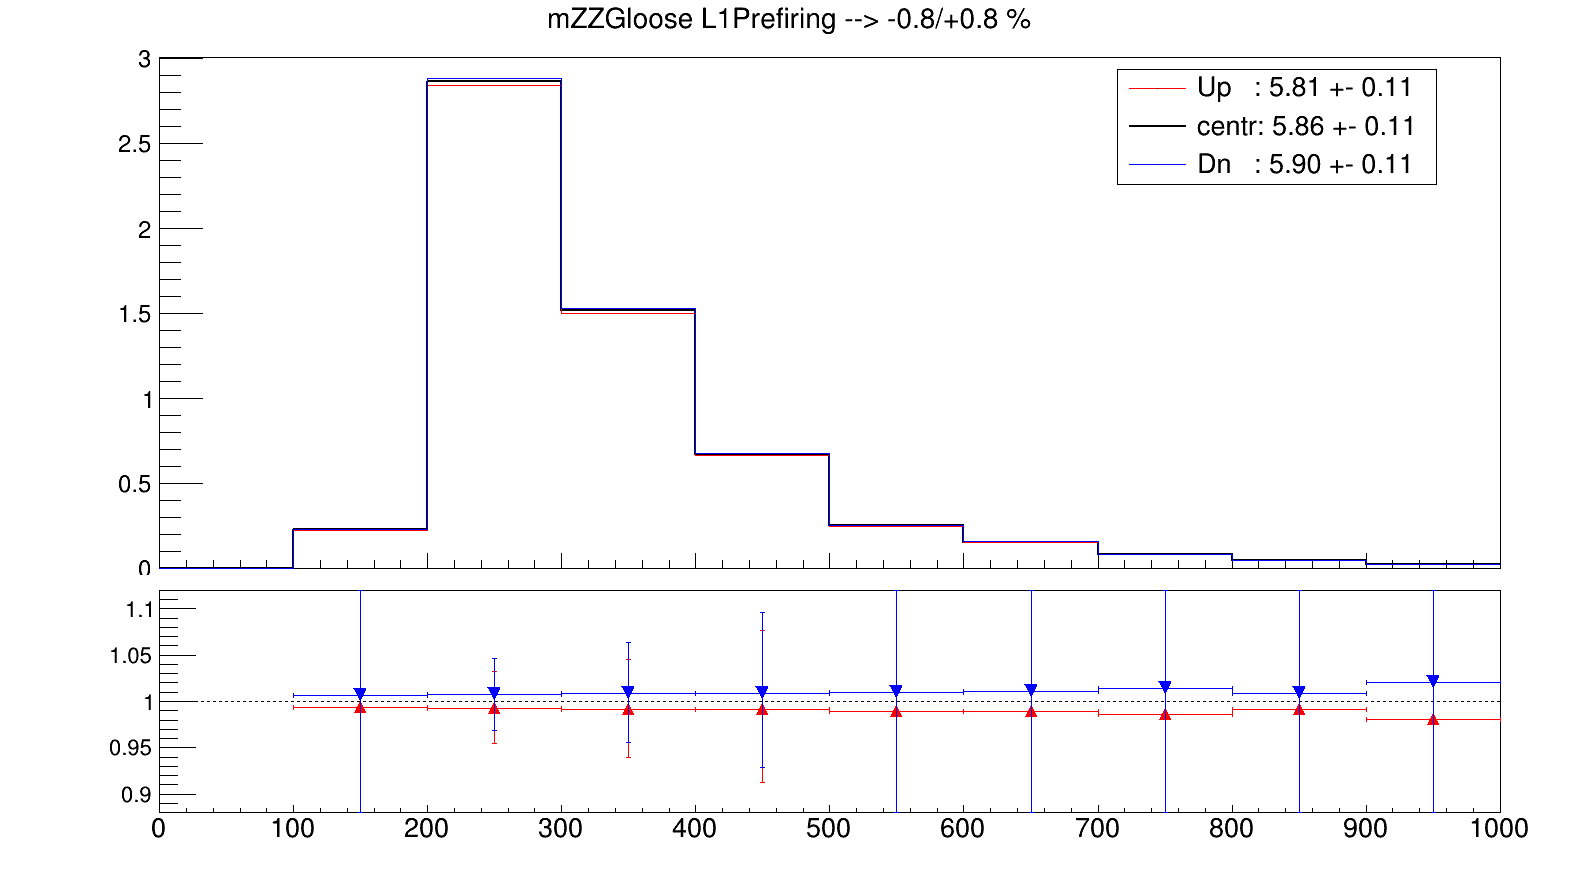
\includegraphics[width=.5\textwidth]{Figures/SYS/SR4P/ZZGTo4LG_mZZGloose_L1Prefiring.png}}}
\caption{L1 pre-firing weights and effect of their application on the signal MC in the region SR4P\_P in 2018. The photon is required to pass the Loose cut-based ID}
\label{fig:L1Prefiring}
\end{figure}

The Fig~\ref{fig:L1Prefiring} shows the impact of the L1 pre-firing weights on the signal MC.
The impact on the normalization of the signal is around 0.8\%.

\paragraph{Removal of noisy jets}

Increased jet multiplicity was reported for 2017 data, creating ``horns'' in the jet $\eta$ distribution for $2.5<|\eta_{jet}|<3$.
The issue was linked to an increase of the ECAL noise, PU and bunch-crossing dependent, thus getting worse as luminosity increases.
The problem can only be fixed in the UL ReReco.
For now, we checked the impact of rejecting jets with raw $p_T<50$ GeV in 2.65 $<|\eta| <$ 3.139.
As we see no significant impact in the data/MC agreement, we decided not to use these cuts.

%\paragraph{HEM 15/16 failures}

%Following	a CMS-wide power interlock on June 30, the power-on of CAEN A3100HBP modules that provide low-voltage power to the on-detector HE front-end electronics led to irreversible damage of two sectors on the HE minus side, HEM15 and HEM16 (FIXME: add ref). No significant impact was seen and nothing particular is done to cope with this. 

%https://twiki.cern.ch/twiki/bin/view/CMS/HIGJetMET#Known_JetMET_issues 




